\section{Design and Implementation}
\label{sec:design_and_implementation}

In this section, the design and implementation stages were discussed. The fact that we combine the design and implementation stage is because we use agile method to develop the system prototype. At first, we refine our system architecture to have clear structure of the system, that will be explained in \ref{subsec:system_architecture}, to make the development process much easier. After that, the structure and behaviour of each component were refined. This part are clarified in incoming subsection.

\subsection{System Architecture}
\label{subsec:system_architecture}
\begin{figure}[ht]
    \centering
    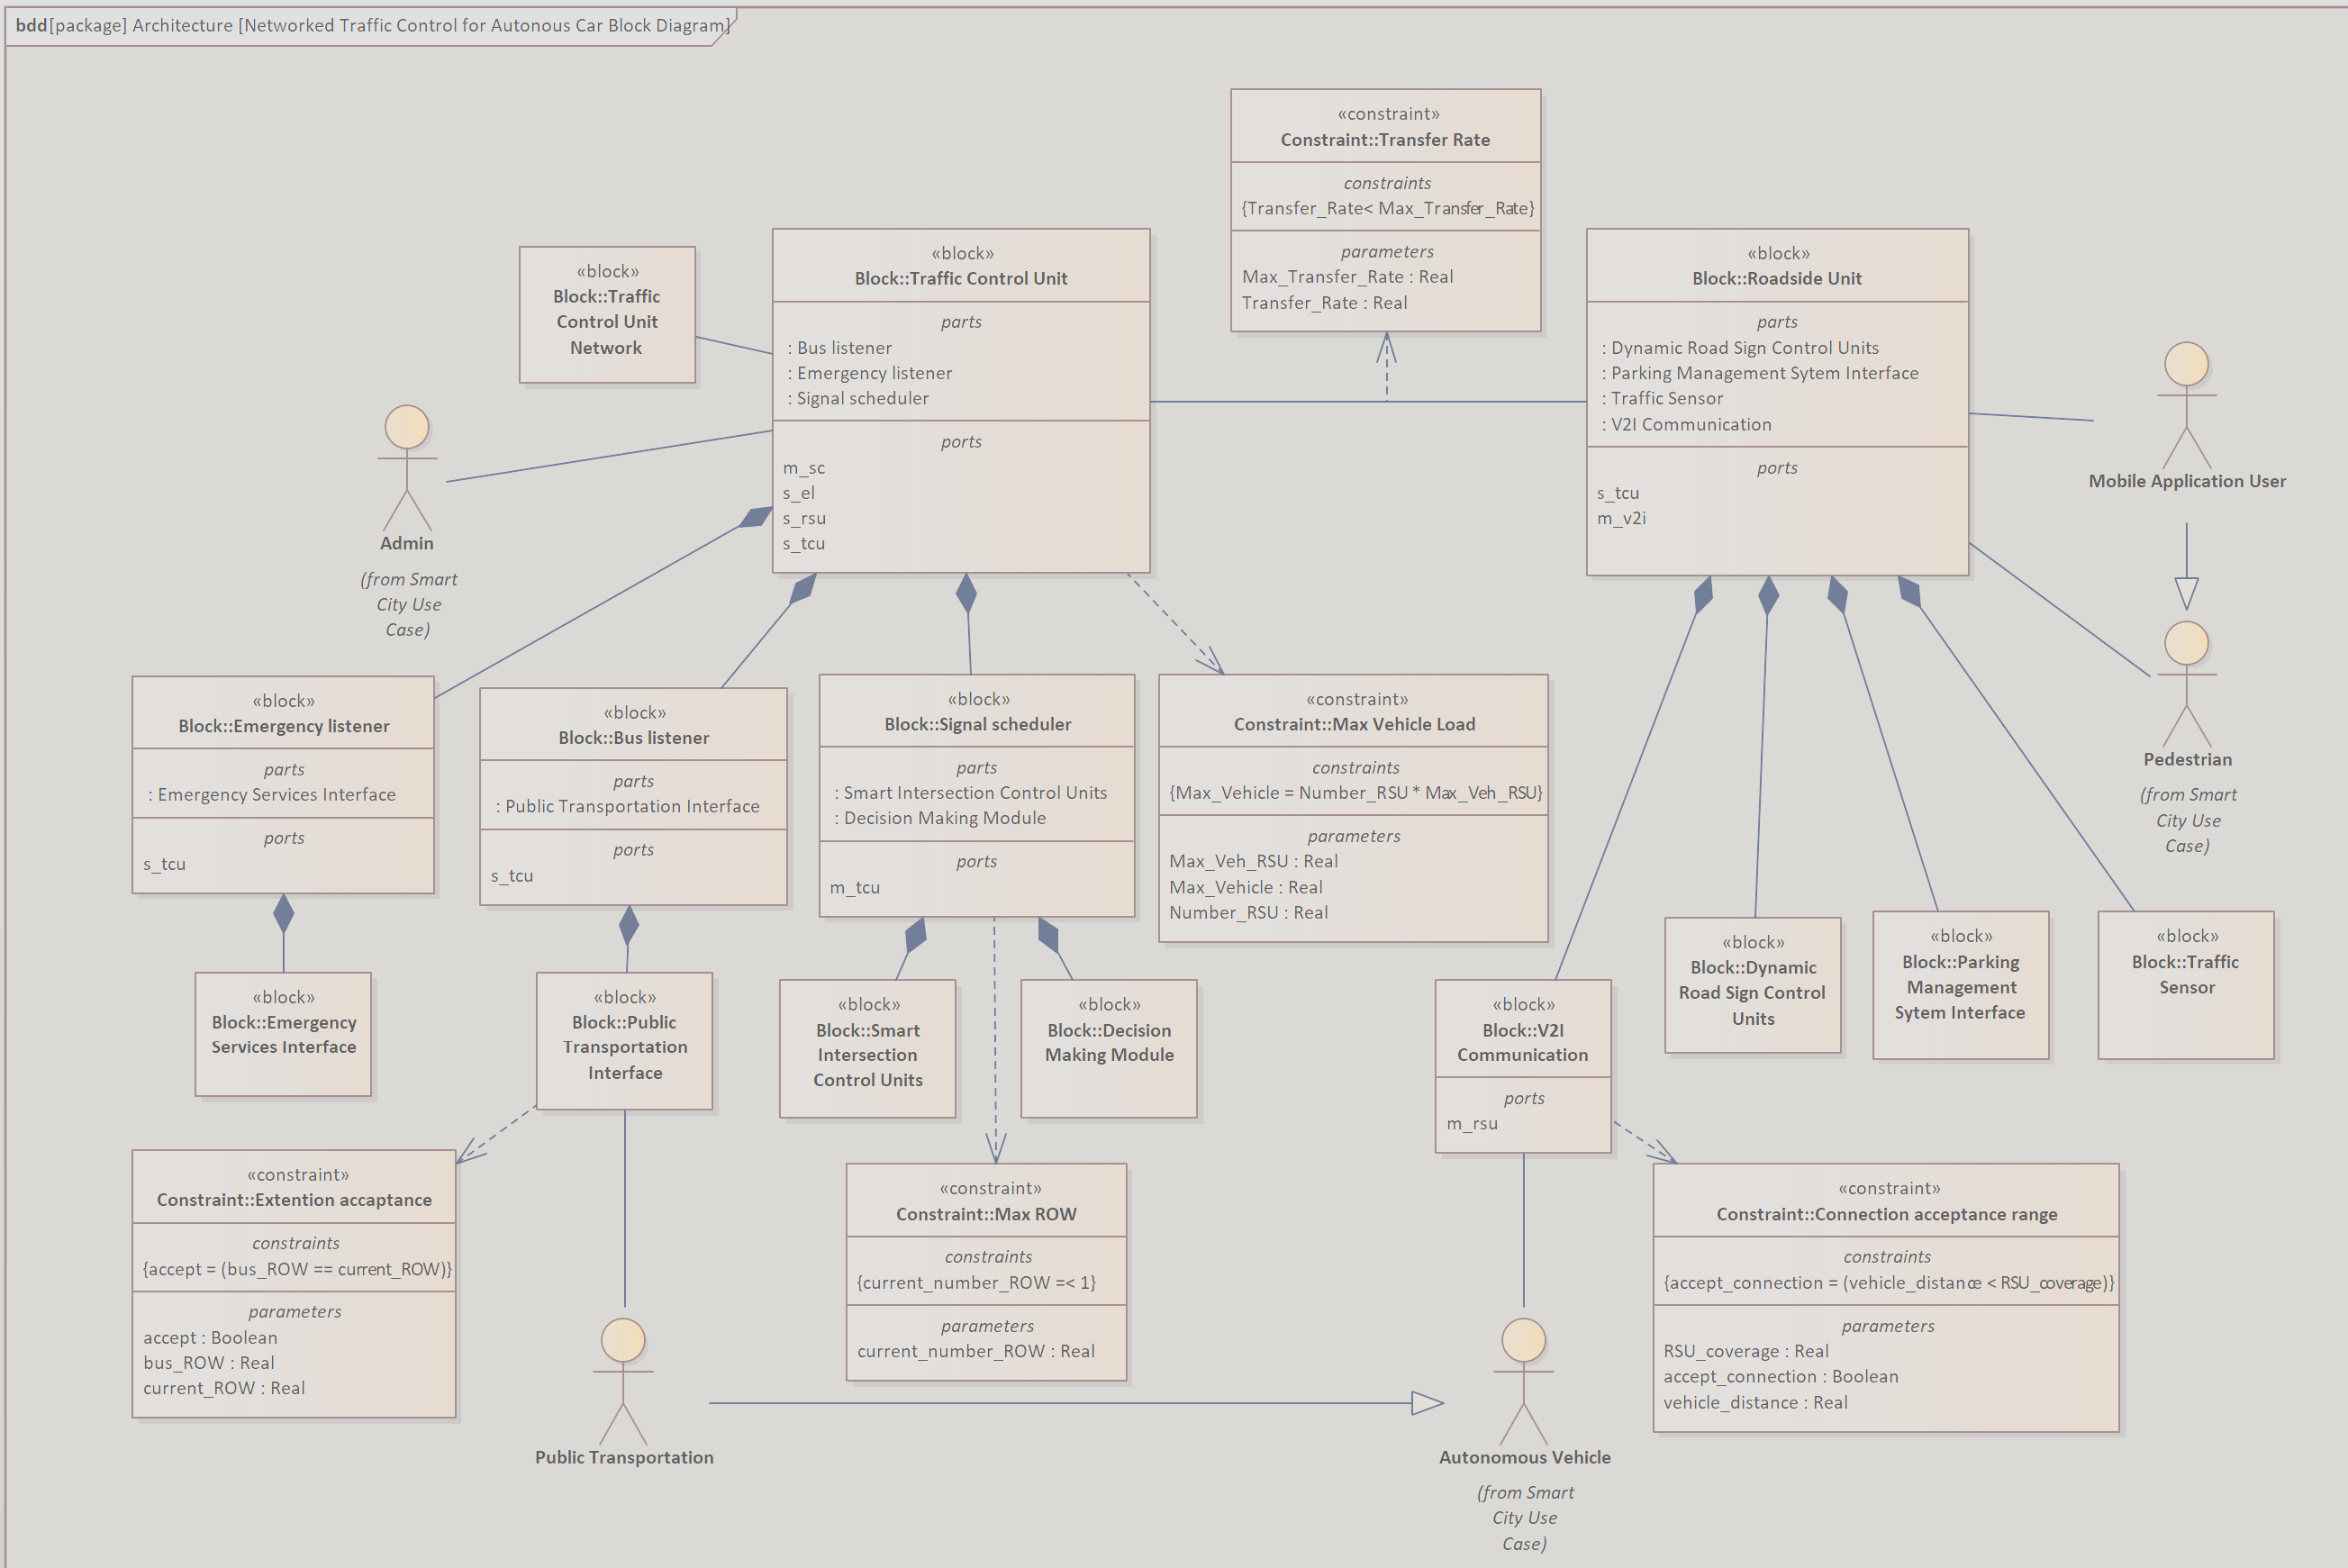
\includegraphics[width=0.5\textwidth]{images/system_bdd.png}
    \caption{System Block Diagram }
    \label{img:system_bdd}
\end{figure}
The architecture in Figure \ref{img:system_bdd} shows the networked traffic control system for autonomous vehicle. It describes how different components and sub-components work together to achieve specific functionalities. There are two main components in our system, TCU(Traffic Control Unit) and RSU(Roadside Unit). TCU control the traffic signals and communicate with traffic through RSU. Further working of both of these components are discussed in below sub-section in this paper. We are considering three main scenarios which are: Bus Listener, Emergency Listener and Signal Scheduler.
Bus Listener receives and processes signals from the buses and the bus stop sign information sensor. It determines the arrival and departure times of the buses and adjusts the traffic signals accordingly.
Emergency Listener handles emergency signals from the emergency vehicle information sensor. It gives priority to the emergency vehicles and alerts  the RSU about the emergency situation.
Signal Scheduler schedules the traffic signals based on certain criteria, such as traffic density, time of day, weather conditions, etc. It also communicates with the signal mixing module and the RSU to coordinate the traffic signals.



